\documentclass{article}

\usepackage[utf8]{inputenc}
\usepackage{url}
\usepackage{graphicx}

\title{FIR Filter Analysis for Accelerometer}
\author{David Lavoie-Boutin\\Malcolm Watt}
\date{\today}

\begin{document}
    \maketitle

    To perform an analysis on which configuration of FIR filter would be optimal for this application, we collected raw accelerometers angles already converted to pitch and roll. We filled a buffer of 1000 elements and imported the data in Matlab. I there, we applied and different filter settings to the data and graphed the output. These are the results we obtained:

    \begin{figure}[!htb]
        \centering
        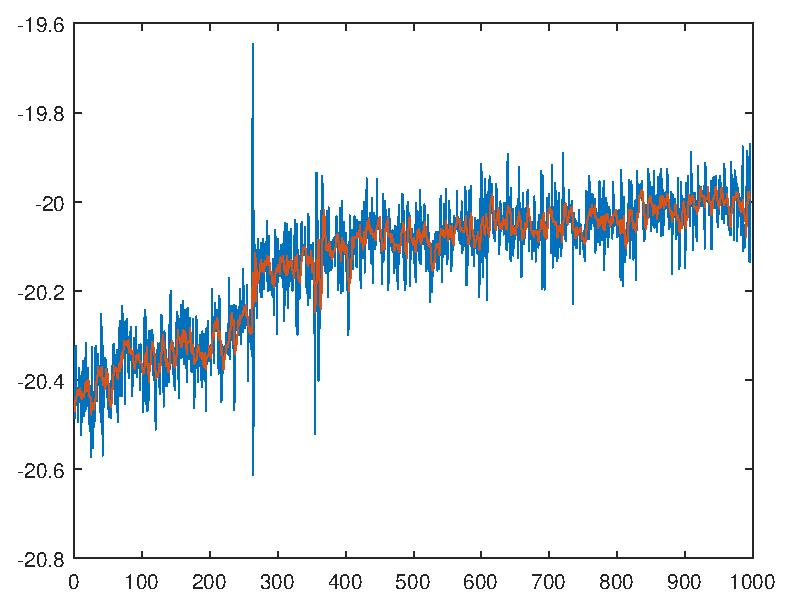
\includegraphics[width = 0.8\textwidth]{../average_size_5.eps}
        \caption{Comparison of raw data with size 5 moving average filter}
    \end{figure}

    \begin{figure}[!htb]
        \centering
        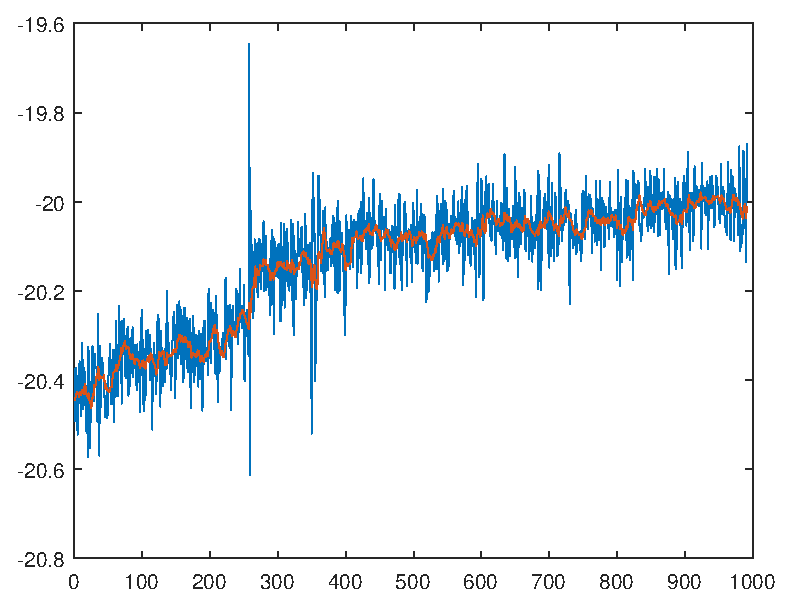
\includegraphics[width = 0.8\textwidth]{../average_size_10.eps}
        \caption{Comparison of raw data with size 10 moving average filter}
    \end{figure}


    \begin{figure}[!htb]
        \centering
        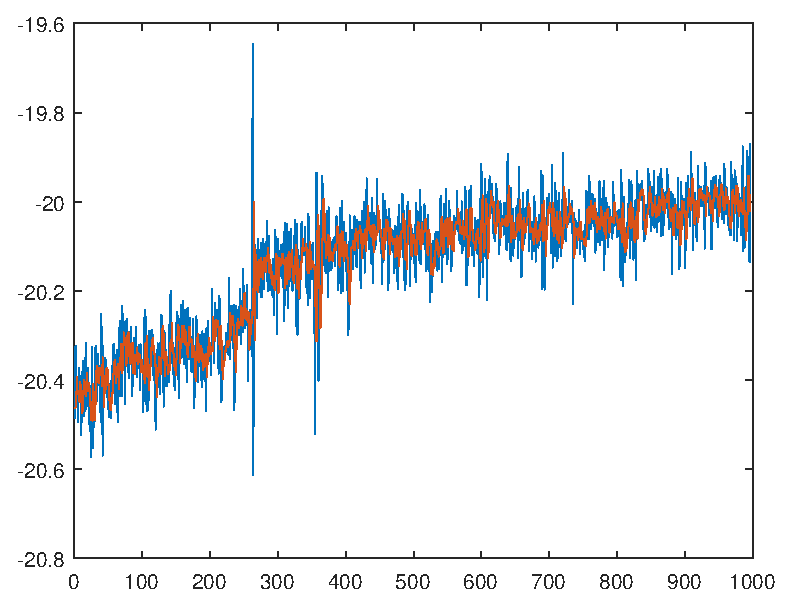
\includegraphics[width = 0.8\textwidth]{../weighted_average_5.eps}
        \caption{Comparison of raw data with size 5 weighted average filter}
    \end{figure}

\clearpage

    From the graphs above, we can see that the weighted average does a very poor job of filtering out the noise. When comparing the results obtained with the 5 and 10 wide window, we do not see a clear best result. The readings from the 10 wide filter are smoother, but there is a significant latency added. On the other hand, the 5 wide filter is faster to respond, but not that unstable. 
    \\
    \\
    For those reasons, we elected to use a moving average filter with a window size of 5 elements.
\end{document}

